\let\negmedspace\undefined
\let\negthickspace\undefined
\documentclass[journal]{IEEEtran}
\usepackage[a5paper, margin=10mm, onecolumn]{geometry}
%\usepackage{lmodern} % Ensure lmodern is loaded for pdflatex
\usepackage{tfrupee} % Include tfrupee package

\setlength{\headheight}{1cm} % Set the height of the header box
\setlength{\headsep}{0mm}     % Set the distance between the header box and the top of the text
\usepackage{gvv-book}
\usepackage{gvv}
\usepackage{cite}
\usepackage{amsmath,amssymb,amsfonts,amsthm}
\usepackage{algorithmic}
\usepackage{graphicx}
\usepackage{textcomp}
\usepackage{xcolor}
\usepackage{txfonts}
\usepackage{listings}
\usepackage{enumitem}
\usepackage{mathtools}
\usepackage{gensymb}
\usepackage{comment}
\usepackage[breaklinks=true]{hyperref}
\usepackage{tkz-euclide} 
\usepackage{listings}
% \usepackage{gvv}                                        
\def\inputGnumericTable{}                                 
\usepackage[latin1]{inputenc}                                
\usepackage{color}                                            
\usepackage{array}                                            
\usepackage{longtable}                                       
\usepackage{calc}                                             
\usepackage{multirow}                                         
\usepackage{hhline}                                           
\usepackage{ifthen}                                           
\usepackage{lscape}
\begin{document}

\bibliographystyle{IEEEtran}
\vspace{3cm}

\title{Scientific Calculator}
\author{EE24BTECH11027 - satwikagv}
% \maketitle
% \newpage
% \bigskip
{\let\newpage\relax\maketitle}

\renewcommand{\thefigure}{\theenumi}
\renewcommand{\thetable}{\theenumi}
\setlength{\intextsep}{10pt} % Space between text and floats


\numberwithin{equation}{enumi}
\numberwithin{figure}{enumi}
\renewcommand{\thetable}{\theenumi}

\section*{\textbf{Objective}}
The goal is to design a scientific calculator using an Arduino and an LCD display. The calculator should support basic arithmetic and scientific functions such as sine, cosine, and their inverses and logarithm.
\section*{\textbf{Hardware Required}}
\begin{itemize}
    \item Arduino Uno
    \item 16X2 LCD display
    \item Bread Board 
    \item Push Buttons
    \item Connecting wires
    \item A Resistor of 220$\Omega$
\end{itemize}
\section*{\textbf{Circuit Design}}
\begin{itemize}
    \item Connect the following 
\begin{table}[h]
\centering
%\caption{Connection Details}
\begin{tabular}{|l|l|}
\hline
\textbf{LCD} & \textbf{Connection} \\ \hline
1 & GND \\ \hline
2 & 5V \\ \hline
3 & potentiometer (middle) \\ \hline
4 & 12 \\ \hline
5 & GND \\ \hline
6 & 11 \\ \hline
11 & 5 \\ \hline
12 & 4 \\ \hline
13 & 3 \\ \hline
14 & 2 \\ \hline
15 & 5V \\ \hline
16 & GND \\ \hline
\end{tabular}
\quad
\begin{tabular}{|l|l|}
\hline
\textbf{Buttons} & \textbf{Connection} \\ \hline
1 & 13 \\ \hline
2 & 6 \\ \hline
3 & 7 \\ \hline
4 & 8 \\ \hline
5 & 9 \\ \hline
6 & 10 \\ \hline
7 & A0 \\ \hline
8 & A1 \\ \hline
9 & A2 \\ \hline
10 & A3 \\ \hline
11 & A4 \\ \hline
12 & A5 \\ \hline
\end{tabular}
\end{table}\\
\item The button 1 represents the right toggle button and the button 12 represents left toggle button.
\item The rest represents different functions when toggled and normally it represents from 0-9 in order.
\end{itemize}
\begin{figure}[H]
    \centering
    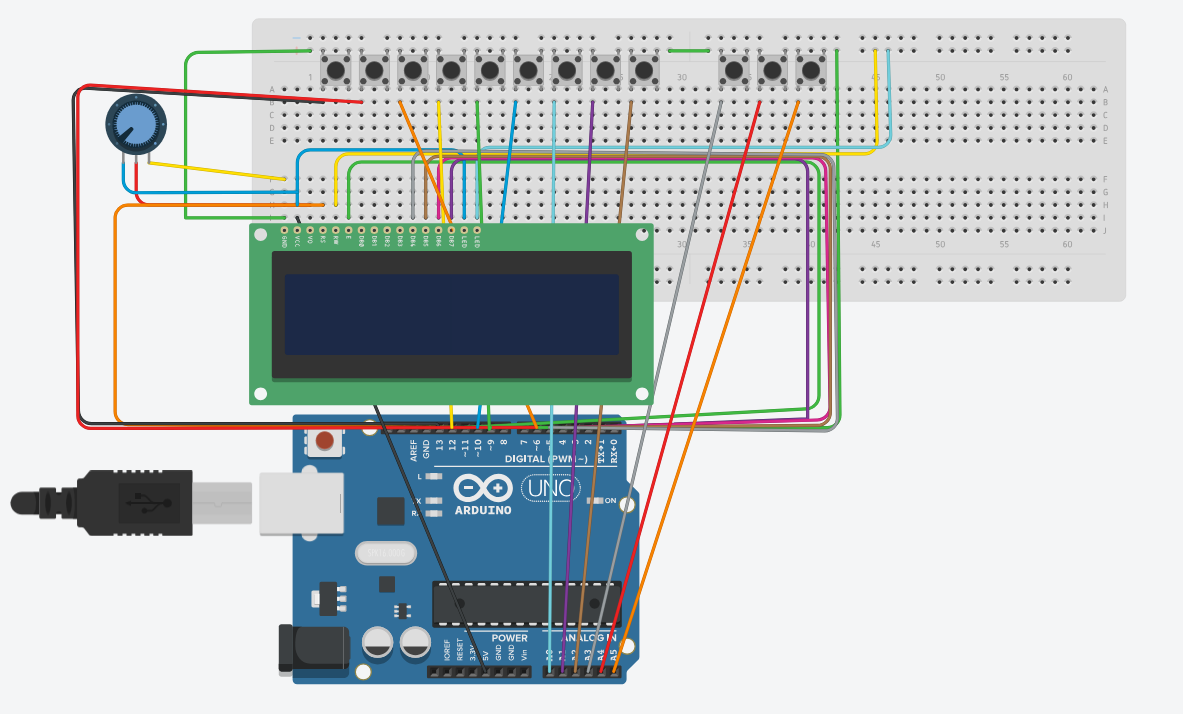
\includegraphics[width=0.8\linewidth]{figs/calcicircuit.png}
\end{figure}
\subsection*{\textbf{Button representing Functions:}}
\begin{tabular}{|l|l|l|}
\hline
\textbf{Button} & \textbf{Right Toggle} & \textbf{Left Toggle} \\ \hline
     2 &  + & $sin^{-1}x$ \\ \hline
     3 &  - & $cos^{-1}x$ \\ \hline
     4 &  * & $tan^{-1}x$ \\ \hline
     5 &  / & $log_{10}x$ \\ \hline
     6 & = & lnx \\ \hline
     7 & backspace & \\ \hline
     8 & sinx & \\ \hline
     9 & cosx & \\ \hline
     10 & $e^x$ & \\ \hline
     11 & $\sqrt{x}$ & \\ \hline 
\end{tabular}\\
After Upload the following code to the Arduino Uno.Refer to the file \texttt{codes/main.c}.

\section*{\textbf{Implementation} }
\begin{itemize}
    \item \textbf{Toggle input Mechanism:} Instead of a matrix keypad, two toggle buttons (right toggle and left toggle) are used for selecting input values and operations.
    \item \textbf{Display handling :}The LCD display is controlled using the Arduino to show current input, operations, and results.
    \item \textbf{Arithmetic and Scientific Functions:}\\
    \begin{itemize}
        \item Addition, subtraction, multiplication, and division are implemented in AVR assembly.
        \item The trigonometric functions and logarithm functions are computed using differential equations.
    \end{itemize}
    \item \textbf{Input Selection:}\\
    \begin{itemize}
        \item Right toggle moves the selection forward through available numbers and operations.
        \item Left toggle moves the selection backward through available numbers and operations.
    \end{itemize}
    \item \textbf{Result Calculation:}Once the input is confirmed, the Arduino processes the selected operation and displays the result on the LCD.
\end{itemize}

\section*{\textbf{Challenges and Solutions}}
\begin{itemize}
    \item \textbf{Limited input Mechanism:} Overcame the lack of a keypad by using toggle buttons for sequential selection.
    \item \textbf{Handling Complex Calculations:} Used differential equations to compute trigonometric functions and logarithms.
    \item \textbf{Efficient Result Display :} Managed LCD updates to ensure smooth transitions between inputs and results.
\end{itemize}
\section*{\textbf{Conclusion}}
The AVR-based scientific calculator successfully demonstrates:
\begin{itemize}
    \item Integration of multiple hardware components
    \item Implementation of complex mathematical functions on limited hardware
    \item User interface design for embedded systems
    \item Numerical methods for function approximation
\end{itemize}
\end{document}

